\chapter{Descripción de la solución propuesta}
\label{ch:solucion_propuesta}

\section{Aplicación móvil}

La aplicación móvil a desarrollar será una aplicación nativa de Android desarrollada con la última versión de Kotlin estable al momento de comienzo del desarrollo, \textbf{Kotlin 1.5.0}. El código Kotlin será compilado con la \acrshort{jvm} 1.8 como destino. El \acrshort{sdk} de Android objetivo de la aplicación será el SDK 31, kit de desarrollo de la versión más reciente del sistema operativo, Android 12. Sin embargo, el SDK mínimo soportado será el de \textbf{Android 8.1 Oreo} (SDK 26), este abanico equivale a ofrecer un sistema compatible con más del 80\% de dispositivos Android actualmente en el mercado\cite{statcounter2021android}.

\begin{figure}[H]
    \centering
    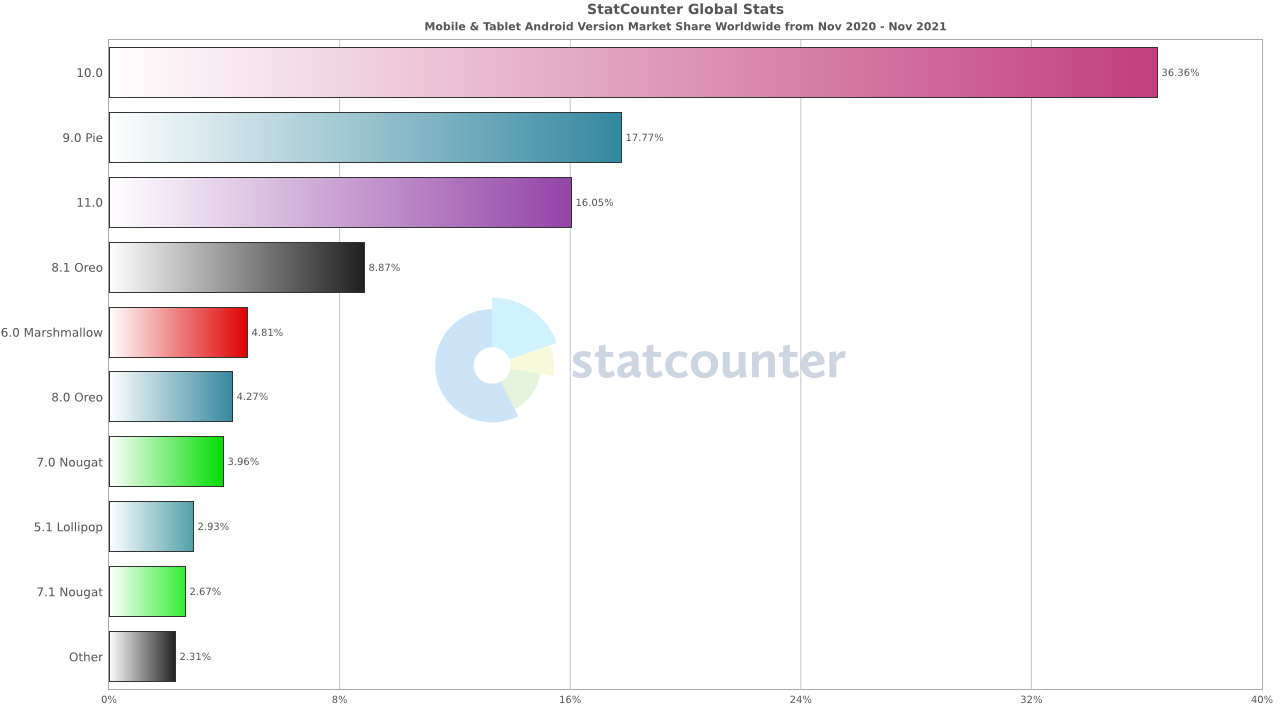
\includegraphics[width=1\textwidth]{images/Introduccion/android-stat.png}
    \caption{Reparto de mercado de Android (nov 20 - nov 21)}
    \label{fig:android-stats}
\end{figure}

Dicho desarrollo se realizará utilizando como herramienta principal el \acrshort{ide} Android Studio. La arquitectura de la aplicación será una \textbf{arquitectura \acrshort{mvvm}}, modelo de arquitectura recomendado actualmente para el desarrollo de aplicaciones Android\cite{mvvm2021}.
Las vistas se realizarán siguiendo las recomendaciones de \textbf{Material Design} (\fref{ssec:guia_material_design}). Las pruebas del sistema se llevarán a cabo con \textbf{JUnit 4} para las pruebas unitarias de componentes y con \textbf{Espresso} para las pruebas de comportamiento de las vistas. 

\subsection{Autenticación}

La autenticación de los usuarios en la aplicación se llevará a cabo siguiendo el protocolo \textbf{OAuth 2.0}\cite{rfc6749}. Dicha autenticación será lograda con apoyo en la \acrshort{api} de autenticación de Google, de esta forma el usuario podrá iniciar sesión con la cuenta Google que ya tiene vinculada al dispositivo o cualquier otra que desee usar. En una primera versión del sistema no se valora añadir otros métodos o vías de autenticación.

\subsection{Geolocalización}

Para la función de geolocalización se hará uso de los dispositivos \acrshort{gps} montados en los terminales de los usuarios. La obtención de la localización y su muestra en un mapa se llevarán a cabo con la \textbf{el kit de desarrollo de mapas de Google} (\ref{lib:app:maps}) para Android. La localización del usuario se comunicará al servidor por vía del WebSocket cuando comience a compartirla, por la misma vía se obtendrá también la localización del resto de usuarios vinculados.

\subsection{Comunicación con la API}

La comunicación por red con la \acrshort{api} se llevará a cabo haciendo uso de la librería \textbf{Retrofit 2} (\fref{lib:app:retrofit2}) de Square Open Source para la realización de peticiones \acrshort{rest}. La comunicación por medio de los WebSockets se llevará a cabo con el \textbf{cliente para Android de Socket.io} (\fref{lib:app:socketio}). El intercambio de datos en ambos protocolos hará uso de Gson\footnote{\href{https://github.com/google/gson}{https://github.com/google/gson}}, la librería de Google para la conversión de objetos Java a \acrshort{json} y viceversa. En los tests la simulación de la comunicación de la \acrshort{api} se realizará con el MockWebServer (\fref{lib:app:mockwebserver}) de Square Open Source.

\subsection{Vinculación de usuarios}

Para la realización de una vinculación de usuarios fiable a la vez que cómoda se realizará por medio del escaneo de códigos QR. Para gestionar la creación y escaneo de los mismos se utilizará \textbf{Zxing}\footnote{\href{https://github.com/zxing/zxing}{https://github.com/zxing/zxing}}, librería de Google para la codificación y decodificación de códigos de barras, códigos QR y similares.

\section{API}

El servidor con la \acrshort{api} y la lógica de negocio del sistema será desarrollada utilizando la última versión estable de Node.js, \textbf{Node v16}\footnote{\href{https://nodejs.org/en/about/releases}{https://nodejs.org/en/about/releases}}. Para fomentar la creación de código más mantenible y resistente a errores se usará como lenguaje de programación \textbf{Typescript} (\fref{lib:typescript}). El código Typescript será compilado a EcmaScript 6\cite{ecma262} con el módulo CommonJS. Para las pruebas se usará la librería \textbf{Jest} (\fref{lib:api:jest}), compatibilizada con Typescript por medio de TSJest (\fref{lib:api:ts_jest}).

El enrutamiento y el manejo de las peticiones \acrshort{http} de la \acrshort{api} \acrshort{rest} será desarrollado y gestionado con la librería \textbf{Express} (\fref{lib:api:express}). Sus pruebas serán manejadas con la librería SuperTest (\fref{lib:api:supertest}). Por otro lado, los WebSockets serán manejados por \textbf{Socket.io} (\fref{lib:api:socket_io}).

\subsection{Autenticación}

La autenticación en el servidor para el uso de la \acrshort{api} \acrshort{rest} será implementado por medio de Bearer tokens\cite{rfc6750}. Se manejarán dos tipos de token. El inicio de sesión se llevará a cabo por medio de \textbf{tokens de autenticación de Google} servidos por la app y que se verificarán por medio de Google Auth Library (\fref{lib:api:google_auth_library}). Una vez iniciada la sesión se proporcionarán tokens de autenticación y refresco para la realización de peticiones privadas a la \acrshort{api} \acrshort{rest}, estos tokens serán \textbf{\acrlong{jwt}}\cite{rfc7519}. La librería de \acrshort{npm}\footnote{Gestor de paquetes de Node.js} de \acrshort{jwt} será la que se usará para la creación, validación y verificación de estos tokens.

\subsection{Persistencia de datos}

La persistencia de datos se realizará con una base de datos documental de MongoDB alojada en la nube en remoto de \textbf{MongoDB Atlas}\footnote{https://www.mongodb.com/atlas/database}. Para el manejo de la base de datos se usará la librería Mongoose (\fref{lib:api:mongoose}). Para utilizarla con todas las fortalezas de Typescript se usará la librería \textbf{Typegoose} (\fref{lib:api:typegoose}). De cara a la ejecución de tests con persistencia se usará la librería de MongoDB Memory Server (\fref{lib:api:inmemory_server}) para replicar la base de datos en memoria.

\section{Despliegue}

La \acrshort{api} del sistema será desplegada en la nube haciendo uso del servicio \textbf{Microsoft Azure}. Puesto que los requisitos de uso del sistema en este proyecto serán mínimos se usará una \textbf{AppService de nivel B1} financiada por el crédito para estudiantes. Para el manejo del despliegue se creará una pipeline de despliegue continuo con GitHub Actions (\fref{tool:github_actions}) que actualice el sistema desplegado cuando se actualice el código de la rama principal del sistema.